% Intended LaTeX compiler: pdflatex
\documentclass{scrartcl}
    \usepackage{amsmath, amssymb, bm}
		\usepackage[utf8]{inputenc}
		\usepackage[dvipdfmx]{graphicx}
		\usepackage[dvipdfmx]{color}
		\usepackage[backend=biber,bibencoding=utf8]{biblatex}
		\usepackage{url}
		\usepackage{indentfirst}
		\usepackage[normalem]{ulem}
		\usepackage{longtable}
		\usepackage{minted}
		\usepackage{fancyvrb}
    \usepackage[dvipdfmx,colorlinks=false,pdfborder={0 0 0}]{hyperref}
    \usepackage{pxjahyper}
    \usepackage{caption}
		\DeclareMathOperator*{\argmax}{argmax}
\DeclareMathAlphabet{\mathpzc}{OT1}{pzc}{m}{it}
\author{情報科学類3年 江畑 拓哉 (201611350)}
\date{}
\title{数理アルゴリズムとシミュレーション\\\medskip
\large 演習課題1}
\begin{document}

\maketitle
\begin{verbatim}
function [] = createGraph(xfrom, xto, m, a)
x = linspace(xfrom, xto, m);
y = zeros(1, m);
n = size(a, 2) - 1;
for i=1:n
    y = (y + a(i)) .* x;
end
y = y + a(n + 1);
plot(x, y)
endfunction
\end{verbatim}


\section{課題1}
\label{sec:orgd2a45dc}
\subsection{}
\label{sec:org758abab}
 次に示す配列 a, b からなるデータ列を配列 a の i 番目の要素 a i を横軸に,配列 b の i 番目の要素 b i を縦軸としたグラフを描画せよ.その際, plot 関数を使うこ\\
と.\\
\begin{verbatim}
plot(a, b)
\end{verbatim}

\begin{center}
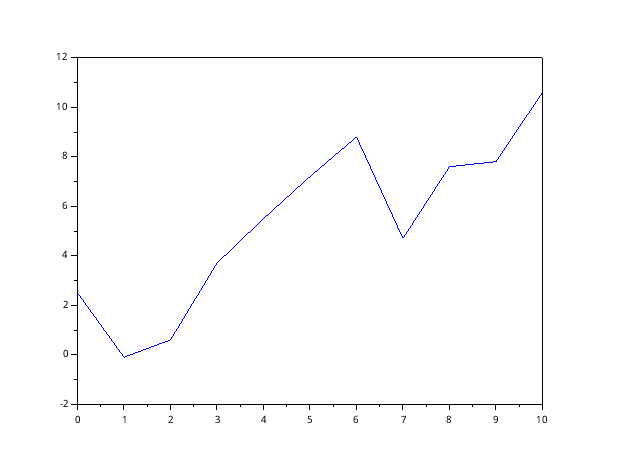
\includegraphics[width=10cm]{./1-1.png}
\end{center}
\subsection{}
\label{sec:org1542e71}
 (1-1) で用いたデータ列を使用して,破線と任意のマーカーを用いてグラフを描画せよ.\\
\begin{verbatim}
plot(a, b, '--*')
\end{verbatim}

\begin{center}
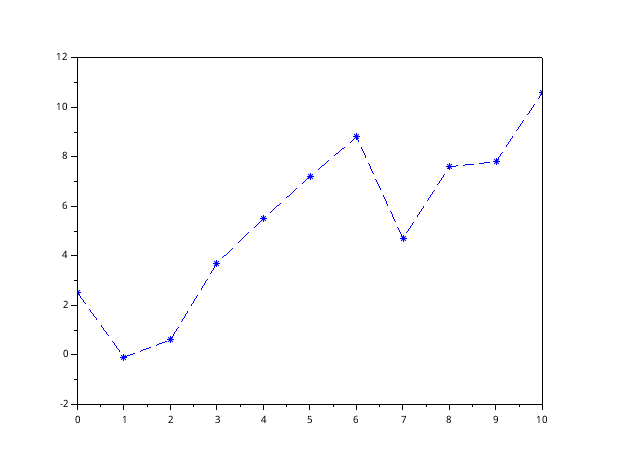
\includegraphics[width=10cm]{./1-2.png}
\end{center}
\subsection{}
\label{sec:org27ab35b}
 (1-2) で描画したグラフに対して,タイトルと軸ラベルを表示せよ.\\
\begin{verbatim}
--> plot(a, b, '--*')

--> title('Plot Test')

--> xlabel('ai')

--> ylabel('bi')
\end{verbatim}

\begin{center}
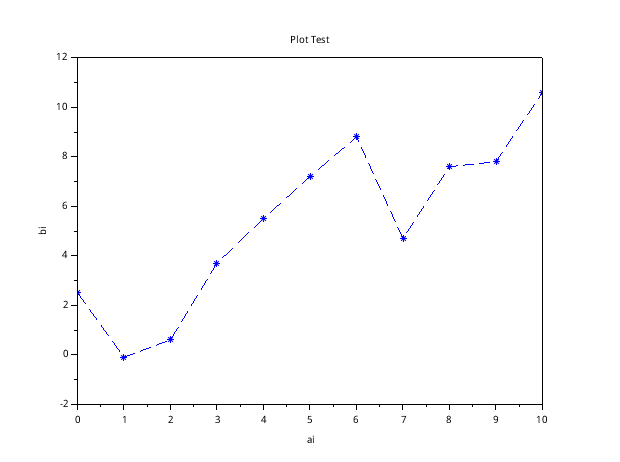
\includegraphics[width=10cm]{./1-3.png}
\end{center}
\section{課題2}
\label{sec:org8e0a32b}
\begin{verbatim}
--> a = [0, 1, 2, 3, 4, 5, 6, 7, 8, 9, 10]
--> b = [0.5, 0.6, 1.5, 1.4, 1.3, 360, 180, 160, 130, 200, 80]
--> plot2d('nn', a, b)
\end{verbatim}

\begin{center}
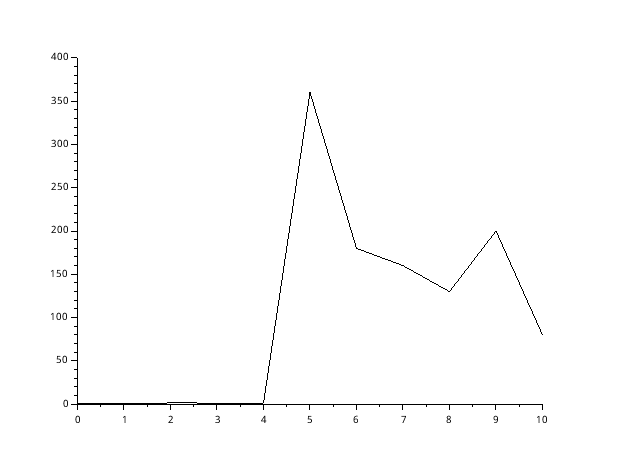
\includegraphics[width=10cm]{./2-no-kata.png}
\end{center}

\begin{verbatim}
--> plot2d('nl', a, b)
\end{verbatim}
\begin{center}
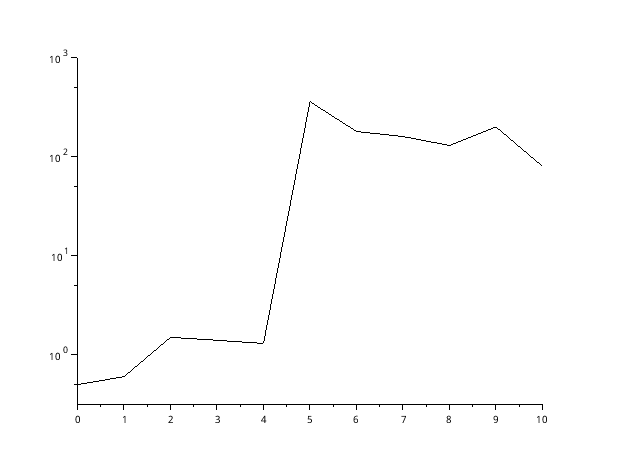
\includegraphics[width=10cm]{./2-kata.png}
\end{center}
\section{課題3}
\label{sec:org2896e15}
\begin{verbatim}
surf(exp(repmat((linspace(-0.5, 0.5, 100))^2, 100, 1) + ..
(repmat((linspace(-0.5, 0.5, 100))^2, 100, 1))'));
\end{verbatim}
\begin{center}
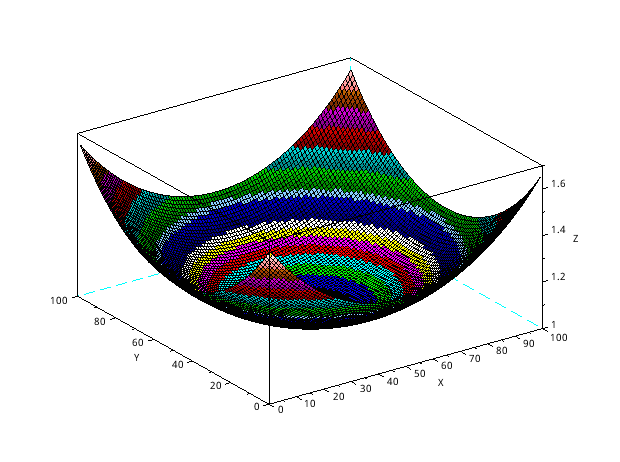
\includegraphics[width=10cm]{./3.png}
\end{center}
\section{課題4}
\label{sec:org303e02b}
\subsection{}
\label{sec:orgba347ed}
\begin{verbatim}
function [] = createGraph(xfrom, xto, m, a)
x = linspace(xfrom, xto, m);
y = zeros(1, m);
n = size(a, 2) - 1;
for i=1:n
    y = (y + a(i)) .* x;
end
y = y + a(n + 1);
plot(x, y)
endfunction
\end{verbatim}
\subsection{}
\label{sec:org1135d22}
\begin{verbatim}
--> createGraph(-3, 3, 30, [-2, 1, 2, 3])
--> createGraph(-4, 4, 30, [0.4, -4.7, 4.1, -4])
\end{verbatim}
\begin{center}
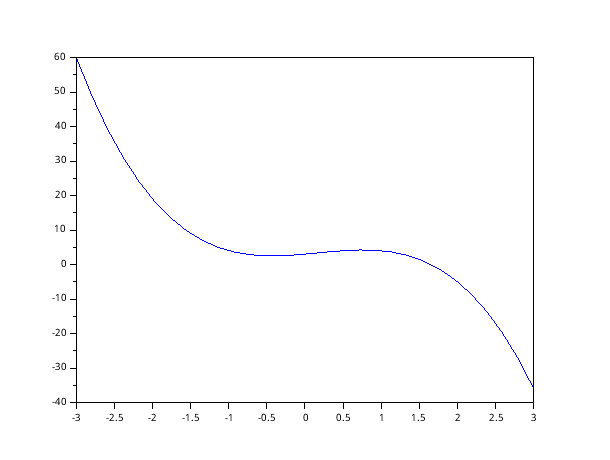
\includegraphics[width=10cm]{./4-1.png}
\end{center}
\begin{center}
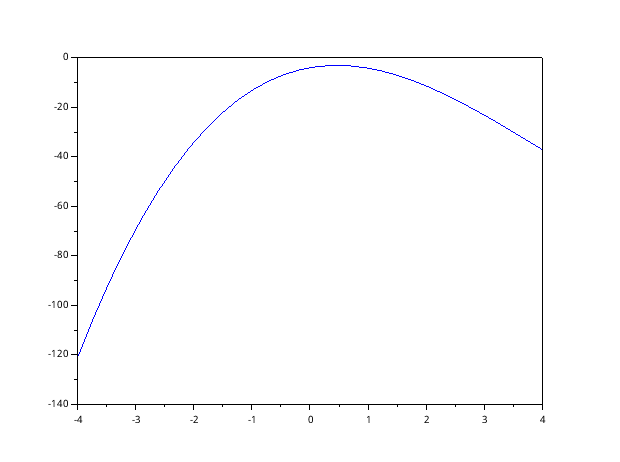
\includegraphics[width=10cm]{./4-2.png}
\end{center}
\end{document}
